\documentclass{standalone}
\usepackage{tikz}
\usetikzlibrary{patterns, positioning}
\usepackage[sfdefault]{ClearSans} %% option 'sfdefault' activates Clear Sans as the default text font
\usepackage[T1]{fontenc}

\begin{document}
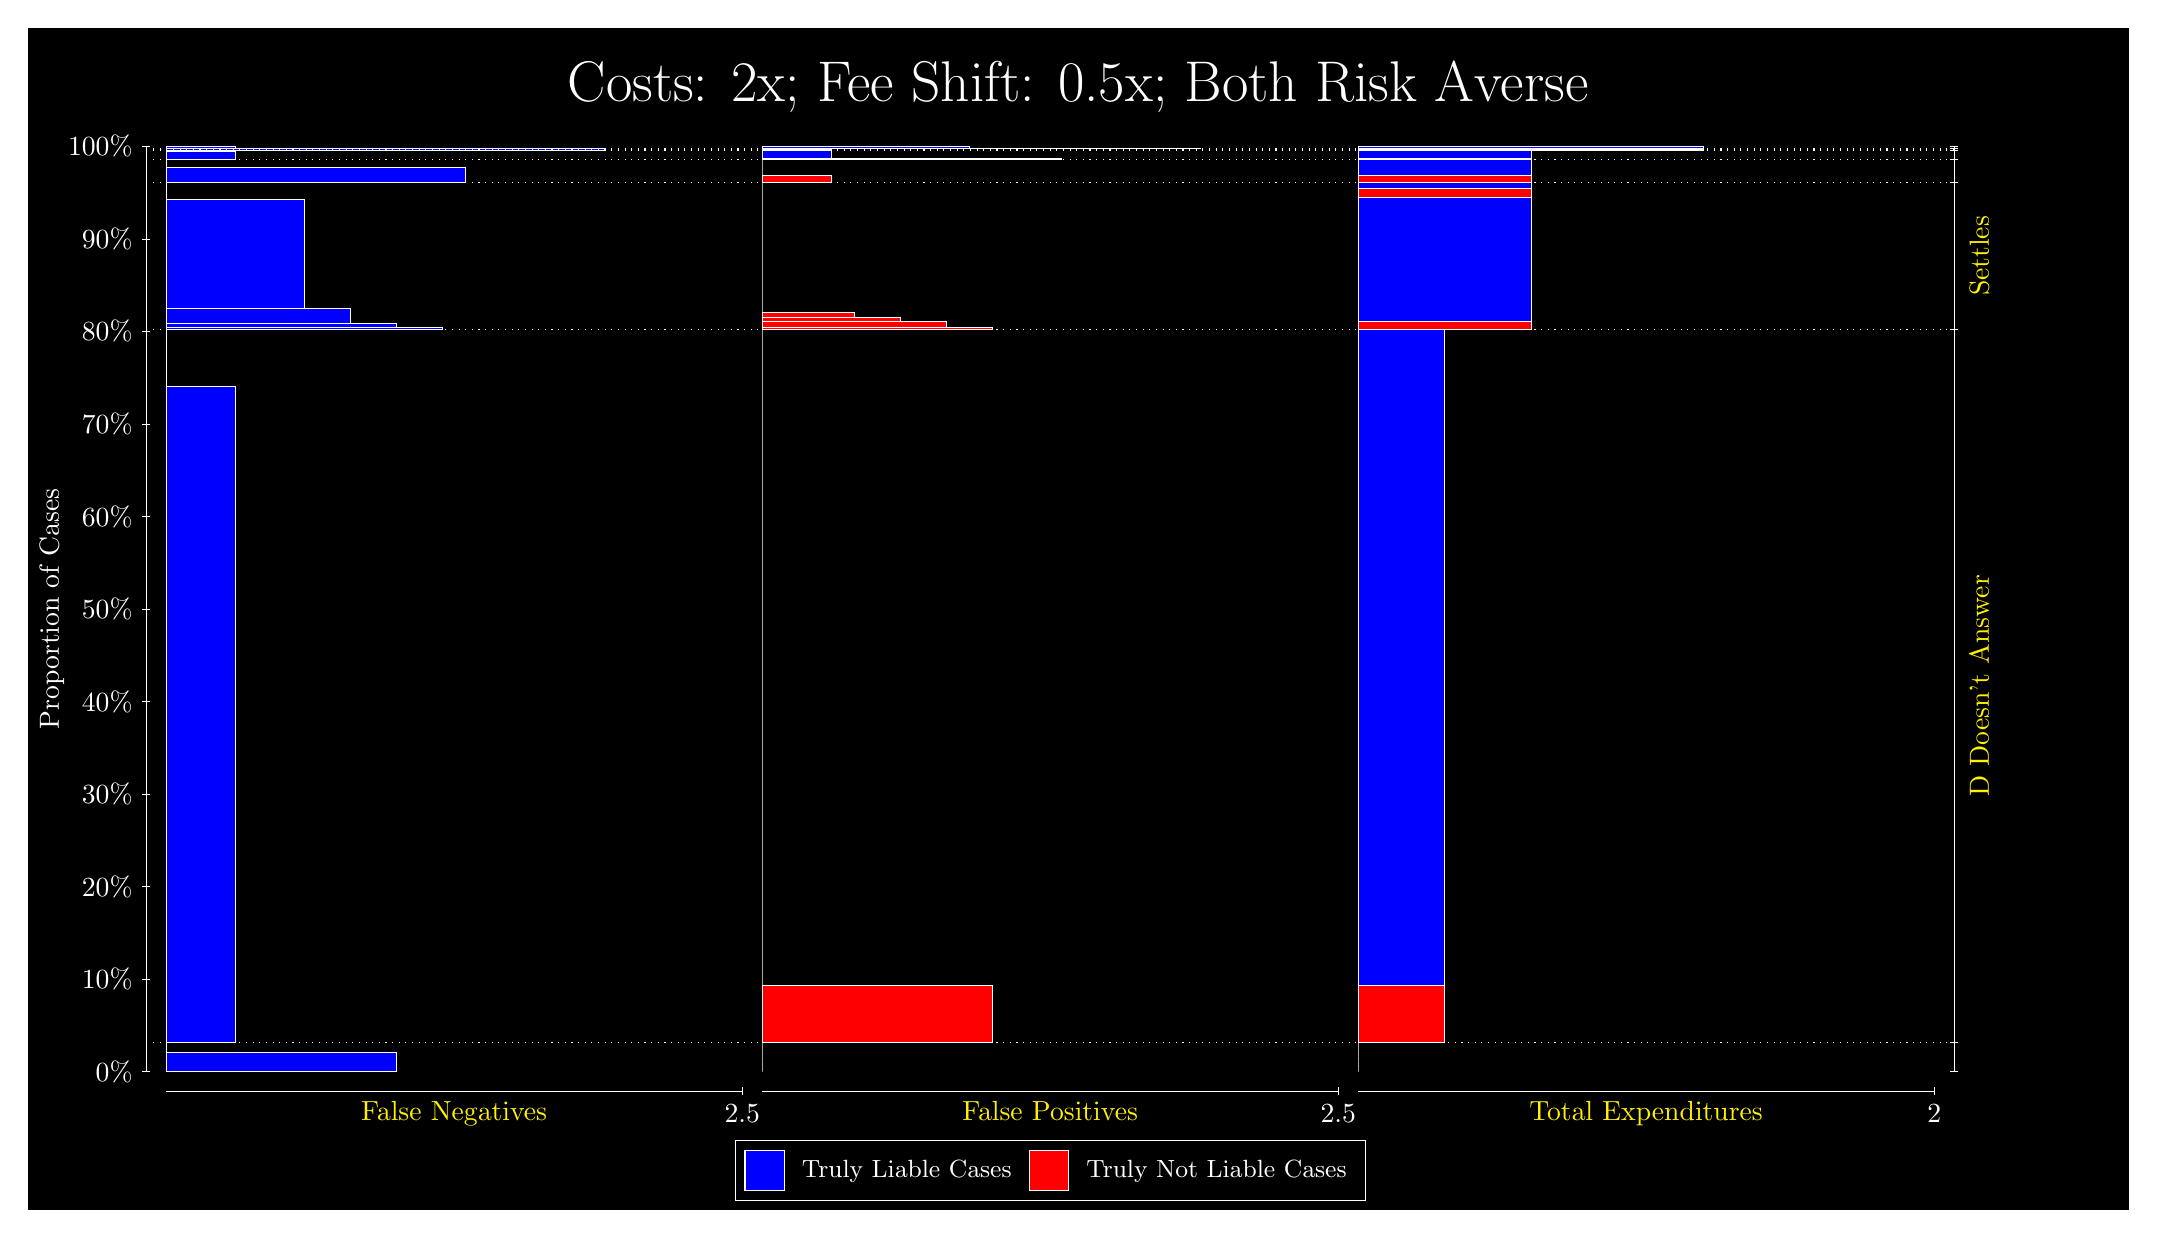
\begin{tikzpicture}
\draw[fill=black] (0,0) rectangle (26.667,15);
\draw[text=white] (0,13.5) rectangle (26.667,15) node[midway] {\huge Costs: 2x; Fee Shift: 0.5x; Both Risk Averse};
\draw[white, very thin] (1.5,1.75) -- (1.5,13.5);
\node[rotate=90, text=white, anchor=center] at (0.3, 7.625) {Proportion of Cases};
\draw[white, very thin] (1.45,1.75) -- (1.55,1.75);
\node[text=white, anchor=east] at (1.45, 1.75) {0\%};
\draw[white, very thin] (1.45,2.925) -- (1.55,2.925);
\node[text=white, anchor=east] at (1.45, 2.925) {10\%};
\draw[white, very thin] (1.45,4.1) -- (1.55,4.1);
\node[text=white, anchor=east] at (1.45, 4.1) {20\%};
\draw[white, very thin] (1.45,5.275) -- (1.55,5.275);
\node[text=white, anchor=east] at (1.45, 5.275) {30\%};
\draw[white, very thin] (1.45,6.45) -- (1.55,6.45);
\node[text=white, anchor=east] at (1.45, 6.45) {40\%};
\draw[white, very thin] (1.45,7.625) -- (1.55,7.625);
\node[text=white, anchor=east] at (1.45, 7.625) {50\%};
\draw[white, very thin] (1.45,8.8) -- (1.55,8.8);
\node[text=white, anchor=east] at (1.45, 8.8) {60\%};
\draw[white, very thin] (1.45,9.975) -- (1.55,9.975);
\node[text=white, anchor=east] at (1.45, 9.975) {70\%};
\draw[white, very thin] (1.45,11.15) -- (1.55,11.15);
\node[text=white, anchor=east] at (1.45, 11.15) {80\%};
\draw[white, very thin] (1.45,12.325) -- (1.55,12.325);
\node[text=white, anchor=east] at (1.45, 12.325) {90\%};
\draw[white, very thin] (1.45,13.5) -- (1.55,13.5);
\node[text=white, anchor=east] at (1.45, 13.5) {100\%};

\draw[white, very thin] (24.457,1.75) -- (24.457,13.5);
\draw[white, very thin] (24.407,1.75) -- (24.507,1.75);
\node[anchor=west] at (24.407, 1.75) {};
\draw[white, very thin] (24.407,2.1209) -- (24.507,2.1209);
\node[anchor=west] at (24.407, 2.1209) {};
\draw[white, very thin] (24.407,11.171) -- (24.507,11.171);
\node[anchor=west] at (24.407, 11.171) {};
\draw[white, very thin] (24.407,13.044) -- (24.507,13.044);
\node[anchor=west] at (24.407, 13.044) {};
\draw[white, very thin] (24.407,13.332) -- (24.507,13.332);
\node[anchor=west] at (24.407, 13.332) {};
\draw[white, very thin] (24.407,13.453) -- (24.507,13.453);
\node[anchor=west] at (24.407, 13.453) {};
\draw[white, very thin] (24.407,13.473) -- (24.507,13.473);
\node[anchor=west] at (24.407, 13.473) {};
\draw[white, very thin] (24.407,13.5) -- (24.507,13.5);
\node[anchor=west] at (24.407, 13.5) {};

\draw[white, very thin, fill=blue] (1.75,1.75) rectangle (4.6775,1.9918);
\draw[white, very thin, fill=red] (1.75,1.9918) rectangle (1.75,2.1209);
\draw[white, very thin, fill=blue] (1.75,2.1209) rectangle (2.6283,10.45);
\draw[white, very thin, fill=red] (1.75,10.45) rectangle (1.75,11.171);
\draw[white, very thin, fill=blue] (1.75,11.171) rectangle (5.2631,11.208);
\draw[white, very thin, fill=blue] (1.75,11.208) rectangle (4.6775,11.254);
\draw[white, very thin, fill=blue] (1.75,11.254) rectangle (4.092,11.442);
\draw[white, very thin, fill=blue] (1.75,11.442) rectangle (3.5065,12.828);
\draw[white, very thin, fill=red] (1.75,12.828) rectangle (1.75,13.044);
\draw[white, very thin, fill=blue] (1.75,13.044) rectangle (5.5558,13.239);
\draw[white, very thin, fill=red] (1.75,13.239) rectangle (1.75,13.332);
\draw[white, very thin, fill=blue] (1.75,13.332) rectangle (2.6283,13.443);
\draw[white, very thin, fill=red] (1.75,13.443) rectangle (1.75,13.453);
\draw[white, very thin, fill=blue] (1.75,13.453) rectangle (7.3123,13.469);
\draw[white, very thin, fill=red] (1.75,13.469) rectangle (1.75,13.473);
\draw[white, very thin, fill=blue] (1.75,13.473) rectangle (2.6283,13.498);
\draw[white, very thin, fill=red] (1.75,13.498) rectangle (1.75,13.5);
\draw[white, very thin, fill=red] (9.3189,1.75) rectangle (9.3189,1.8792);
\draw[white, very thin, fill=blue] (9.3189,1.8792) rectangle (9.3189,2.1209);
\draw[white, very thin, fill=red] (9.3189,2.1209) rectangle (12.246,2.8417);
\draw[white, very thin, fill=blue] (9.3189,2.8417) rectangle (9.3189,11.171);
\draw[white, very thin, fill=red] (9.3189,11.171) rectangle (12.246,11.208);
\draw[white, very thin, fill=red] (9.3189,11.208) rectangle (11.661,11.279);
\draw[white, very thin, fill=red] (9.3189,11.279) rectangle (11.075,11.326);
\draw[white, very thin, fill=red] (9.3189,11.326) rectangle (10.49,11.387);
\draw[white, very thin, fill=blue] (9.3189,11.387) rectangle (9.3189,13.044);
\draw[white, very thin, fill=red] (9.3189,13.044) rectangle (10.197,13.137);
\draw[white, very thin, fill=blue] (9.3189,13.137) rectangle (9.3189,13.332);
\draw[white, very thin, fill=red] (9.3189,13.332) rectangle (13.125,13.342);
\draw[white, very thin, fill=blue] (9.3189,13.342) rectangle (10.197,13.453);
\draw[white, very thin, fill=red] (9.3189,13.453) rectangle (10.197,13.457);
\draw[white, very thin, fill=blue] (9.3189,13.457) rectangle (9.3189,13.473);
\draw[white, very thin, fill=red] (9.3189,13.473) rectangle (14.881,13.474);
\draw[white, very thin, fill=blue] (9.3189,13.474) rectangle (11.954,13.5);
\draw[white, very thin, fill=red] (16.888,1.75) rectangle (16.888,1.8792);
\draw[white, very thin, fill=blue] (16.888,1.8792) rectangle (16.888,2.1209);
\draw[white, very thin, fill=red] (16.888,2.1209) rectangle (17.986,2.8417);
\draw[white, very thin, fill=blue] (16.888,2.8417) rectangle (17.986,11.171);
\draw[white, very thin, fill=red] (16.888,11.171) rectangle (19.083,11.279);
\draw[white, very thin, fill=blue] (16.888,11.279) rectangle (19.083,12.854);
\draw[white, very thin, fill=red] (16.888,12.854) rectangle (19.083,12.962);
\draw[white, very thin, fill=blue] (16.888,12.962) rectangle (19.083,13.044);
\draw[white, very thin, fill=red] (16.888,13.044) rectangle (19.083,13.137);
\draw[white, very thin, fill=blue] (16.888,13.137) rectangle (19.083,13.332);
\draw[white, very thin, fill=red] (16.888,13.332) rectangle (19.083,13.342);
\draw[white, very thin, fill=blue] (16.888,13.342) rectangle (19.083,13.453);
\draw[white, very thin, fill=red] (16.888,13.453) rectangle (21.279,13.457);
\draw[white, very thin, fill=blue] (16.888,13.457) rectangle (21.279,13.473);
\draw[white, very thin, fill=red] (16.888,13.473) rectangle (21.279,13.474);
\draw[white, very thin, fill=blue] (16.888,13.474) rectangle (21.279,13.5);
\draw[white, dotted] (1.5,2.1209) -- (24.457,2.1209);
\draw[white, dotted] (1.5,11.171) -- (24.457,11.171);
\draw[white, dotted] (1.5,13.044) -- (24.457,13.044);
\draw[white, dotted] (1.5,13.332) -- (24.457,13.332);
\draw[white, dotted] (1.5,13.453) -- (24.457,13.453);
\draw[white, dotted] (1.5,13.473) -- (24.457,13.473);
\draw[white, very thin] (1.75,1.5) -- (9.0689,1.5);
\node[text=yellow, anchor=north] at (5.4094, 1.5) {False Negatives};
\draw[white, very thin] (9.0689,1.45) -- (9.0689,1.55);
\node[text=white, anchor=north] at (9.0689, 1.45) {2.5};

\draw[white, very thin] (9.3189,1.5) -- (16.638,1.5);
\node[text=yellow, anchor=north] at (12.978, 1.5) {False Positives};
\draw[white, very thin] (16.638,1.45) -- (16.638,1.55);
\node[text=white, anchor=north] at (16.638, 1.45) {2.5};

\draw[white, very thin] (16.888,1.5) -- (24.207,1.5);
\node[text=yellow, anchor=north] at (20.547, 1.5) {Total Expenditures};
\draw[white, very thin] (24.207,1.45) -- (24.207,1.55);
\node[text=white, anchor=north] at (24.207, 1.45) {2};


\node[text=yellow, centered, rotate=90] at (24.777, 6.6458) {D Doesn't Answer};
\node[text=yellow, centered, rotate=90] at (24.777, 12.108) {Settles};





\draw (12.978300999999998,1.5) node[draw=none] (baseCoordinate) {};
\begin{scope}[align=center]
        \matrix[scale=0.5, draw=white, below=0.5cm of baseCoordinate, nodes={draw}, column sep=0.1cm]{
            \node[rectangle, draw, minimum width=0.5cm, minimum height=0.5cm, fill=blue] {}; &
            \node[draw=none, font=\small, text=white] (B) {Truly Liable Cases}; &
            \node[rectangle, draw, minimum width=0.5cm, minimum height=0.5cm, fill=red] {}; &
            \node[draw=none, font=\small, text=white] (B) {Truly Not Liable Cases}; \\
            };
\end{scope}

\end{tikzpicture}
\end{document}